\section{front-end}

\frame{
    \frametitle{Front-end}
    \framesubtitle{Overview}
    \begin{enumerate}
    \item Error handling within the parser monad
    \item Order of the front-end
    \item Moving functionality from the type-checker to the parser
    \item Normalizing
    \item Type-checking
    \item Codegen interface
    \end{enumerate}
}
\subsection{Error handeling}

\frame{
    \frametitle{Error handeling within the parser monad}
    \begin{multicols*}{3}
    \section{Concat all the errors}
    Concat all the errors
    \begin{enumerate}
    \item Slow
    \item Get all the errors and thus none
    \end{enumerate}

    \columnbreak

    \section{Give only the last viable error.}
    Give only the last viable error
    \begin{enumerate}
    \item Fast
    \item Posability to lose error information
    \item Posability to get incorrect error information
    \end{enumerate}

    \columnbreak

    \section{Priority for errors}
    Priority for errorszz
    \begin{enumerate}
    \item Fast
    \item More accurate error information
    \item Posability to get incorrect error information
    \end{enumerate}
    \end{multicols*}
}

\frame{
    \frametitle{Errors with priority}
    \begin{figure}

        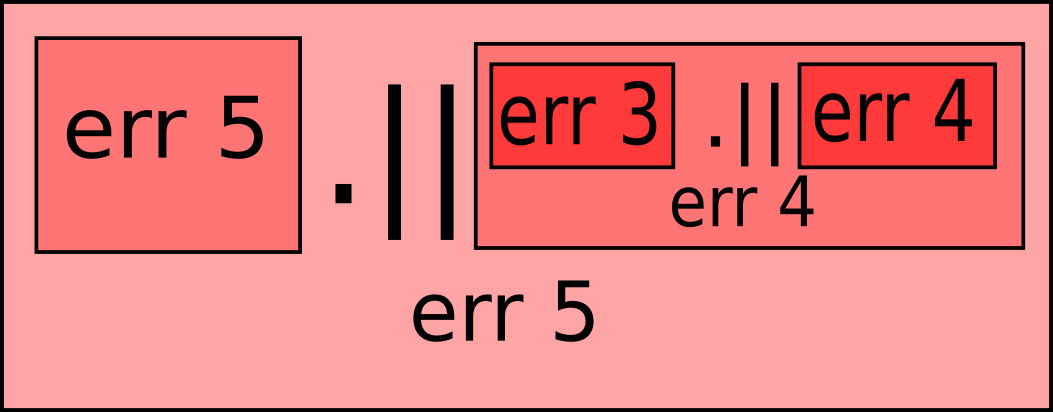
\includegraphics{error_example}
    \end{figure}
}